\section{Resultados y análisis}

Los resultados presentados a continuación corresponden a los tres casos de estudio descritos previamente. El análisis se organiza en torno a la convergencia del algoritmo, la convergencia global e independencia respecto de condiciones iniciales, y la calidad clínica de las soluciones Pareto-óptimas obtenidas.

\subsection{Convergencia del algoritmo}

Para los tres casos, L-BFGS convergió a una solución práctica entre las 300 y 500 iteraciones. Al continuar hasta 5000 iteraciones, los resultados fueron prácticamente idénticos a los obtenidos previamente, lo que indica que el algoritmo no mejora su resultado más allá de ese umbral.

\subsection{Convergencia global}

Para cada caso de estudio se repitió la optimización 100 veces con distintas fluencias iniciales aleatorias, para cada uno de los conjuntos de pesos \(\lambda_m\).

La figura~\ref{fig:convergencia_c} muestra los resultados para el caso fantoma con PTV en forma de C, con 45 conjuntos de pesos distintos (parámetro de muestreo \(k=8\)). Cada punto del eje horizontal representa un conjunto de pesos diferente, correspondiente a un punto distinto del frente de Pareto. Las funciones objetivo individuales (\(F_{\text{PTV}}\), \(F_{\text{NT}}\), \(F_{\text{OAR}}\)) y total (\(F_{\text{tot}}\)) se grafican en escala logarítmica. Al analizar los gráficos, se observa que las 100 distribuciones de resultados para cada conjunto de pesos se superponen completamente, apareciendo como una única curva: esto indica que L-BFGS converge al mismo resultado independientemente de las fluencias iniciales.

\begin{figure}[H]
    \centering
    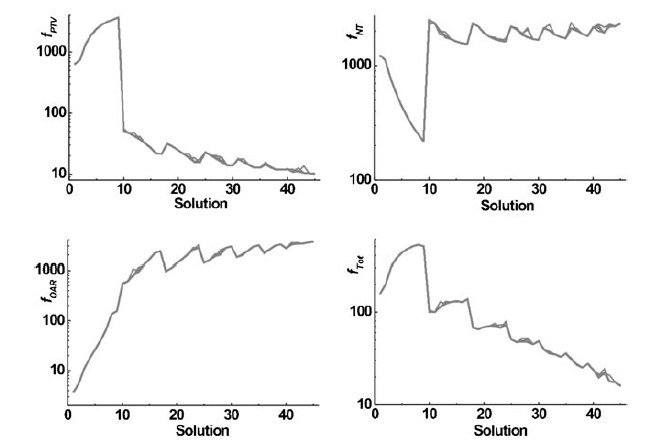
\includegraphics[width=0.75\textwidth]{graficos/Figura_4.PNG}
    \caption{Distribución de las funciones objetivo para 45 soluciones con distintos pesos para el fantoma con PTV en forma de C. Tomado de Lahanas et al.\ (2003).}
    \label{fig:convergencia_c}
\end{figure}
\begin{figure}[H]
    \centering
    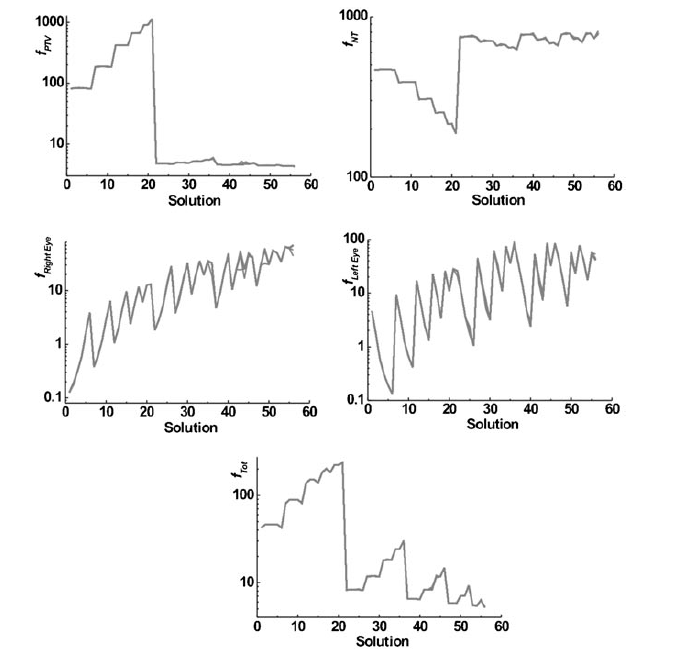
\includegraphics[width=0.75\textwidth]{graficos/Figura_5.PNG}
    \caption{Distribución de las funciones objetivo para 56 soluciones con distintos pesos, caso tumor cerebral. Adaptado de Lahanas et al.\ (2003).}
    \label{fig:convergencia_cerebro}
\end{figure}
\begin{figure}[H]
    \centering
    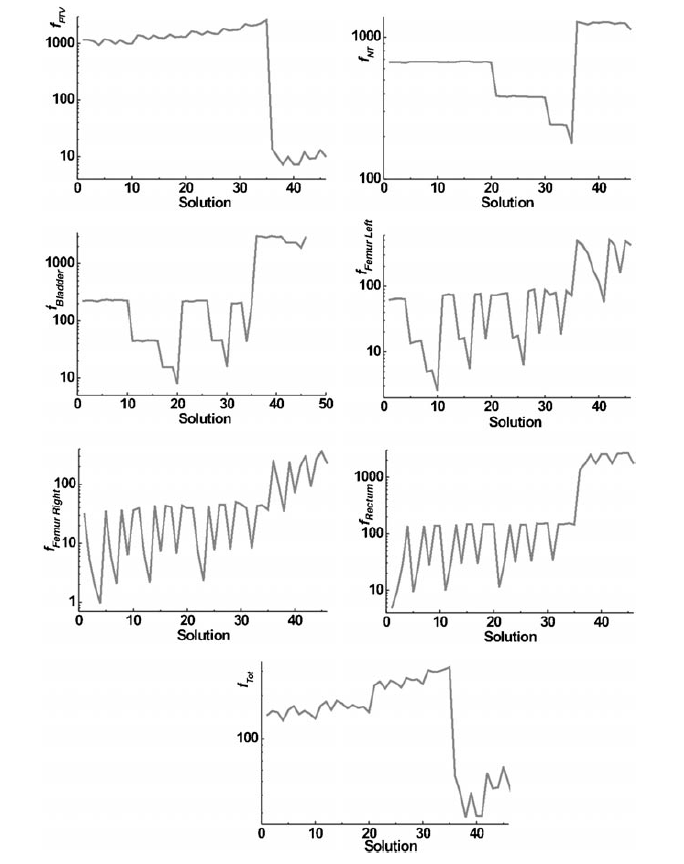
\includegraphics[width=0.8\textwidth]{graficos/Figura_6.PNG}
    \caption{Distribución de los valores de las funciones objetivo para 46 soluciones con distintos conjuntos de pesos, caso cáncer de próstata. Adaptado de Lahanas et al.\ (2003).}
    \label{fig:convergencia_prostata}
\end{figure}

Se observaron resultados similares para el caso de tumor cerebral, mostrados en la figura~\ref{fig:convergencia_cerebro} con 56 conjuntos de pesos (\(k=5\)). En este caso, las funciones objetivo son cinco (PTV, NT, ojo izquierdo, ojo derecho y total), y las 5600 ejecuciones producen distribuciones que a simple vista se superponen en una única curva.

Para el caso de cáncer de próstata, la figura~\ref{fig:convergencia_prostata} muestra los resultados con 46 conjuntos de pesos (\(k=3\)) y hasta 5000 iteraciones por ejecución, con seis estructuras anatómicas. También aquí las 4600 ejecuciones producen resultados independientes de las condiciones iniciales.

El único caso donde se observaron fallas de convergencia global fue el caso con PTV en forma de C, en aproximadamente el 1--2\% de las optimizaciones, donde la función objetivo difirió hasta un 20\% respecto del resultado predominante. La figura~\ref{fig:falla_convergencia} muestra este fenómeno para 400 repeticiones para el OAR. Cada subfigura muestra cómo varía la dosis en el PTV en una escala amplificada. En la figura~\ref{fig:falla_convergencia}(a), con 500 iteraciones y sin corrección, hay picos notables de fluctuación. En la figura~\ref{fig:falla_convergencia}(b), se aumentó a 2000 iteraciones, y se observa que esas soluciones subóptimas mejoran parcialmente pero no desaparecen. En la figura~\ref{fig:falla_convergencia}(c), aplicando el mecanismo de perturbación con sólo 500 iteraciones, todas las soluciones convergen al mismo valor, quedando así demostrada la utilidad de esta herramienta para favorecer la convergencia global del algoritmo.

\begin{figure}[H]
    \centering
    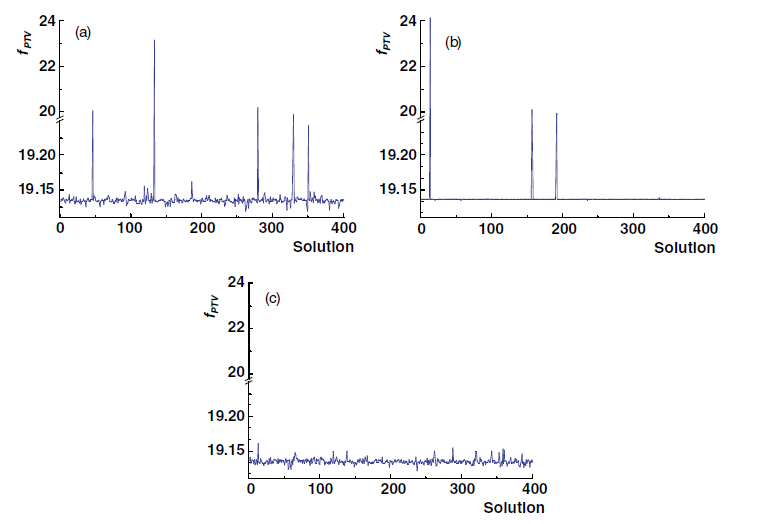
\includegraphics[width=0.85\textwidth]{graficos/Figura_7.PNG}
    \caption{Varianza de dosis en el PTV para 400 soluciones del caso con PTV en forma de C. (a) Sin corrección, 500 iteraciones. (b) Sin corrección, 2000 iteraciones. (c) Con mecanismo de perturbación, 500 iteraciones. Adaptado de Lahanas et al.\ (2003).}
    \label{fig:falla_convergencia}
\end{figure}

\subsection{Comparación con \textit{Simulated Annealing}}

Para verificar que las soluciones de L-BFGS son globalmente óptimas y no mínimos locales, se compararon con las soluciones obtenidas por FSA.

La figura~\ref{fig:lbfgs_vs_fsa_c} muestra la comparación para el caso con PTV en forma de C, graficando los valores de las funciones objetivo obtenidos por L-BFGS (línea continua) y FSA (círculos). Las dos curvas se superponen prácticamente en todos los puntos del frente, lo que indica que L-BFGS y FSA convergen a las mismas soluciones. En base a la garantía teórica de optimalidad global del FSA que fue previamente explidada, queda confirmado que las soluciones de L-BFGS no son mínimos locales sino el mínimo global.

La figura~\ref{fig:lbfgs_vs_fsa_cerebro} muestra la misma comparación pero para el tumor cerebral. En este caso, los autores informan que FSA requirió más de 6 horas y más de 2 millones de iteraciones por optimización, por lo que se utilizó un subconjunto reducido de soluciones para la comparación. Aun así, los puntos de FSA coinciden con la curva de L-BFGS en todas las funciones objetivo, incluyendo las de los dos ojos, que son los que tienen valores más pequeños y por lo tanto una escala que penaliza más las diferencias.

\begin{figure}[H]
    \centering
    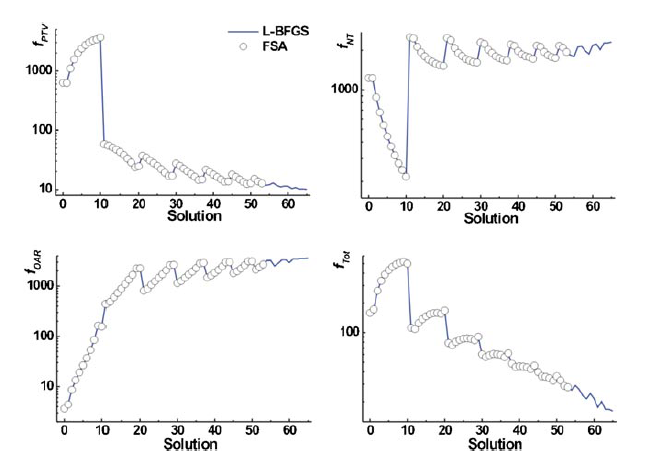
\includegraphics[width=0.8\textwidth]{graficos/Figura_11.PNG}
    \caption{Comparación de los valores de las funciones objetivo individuales y total obtenidos por L-BFGS y FSA para el caso fantoma con PTV en forma de C. Adaptado de Lahanas et al.\ (2003).}
    \label{fig:lbfgs_vs_fsa_c}
\end{figure}

\begin{figure}[H]
    \centering
    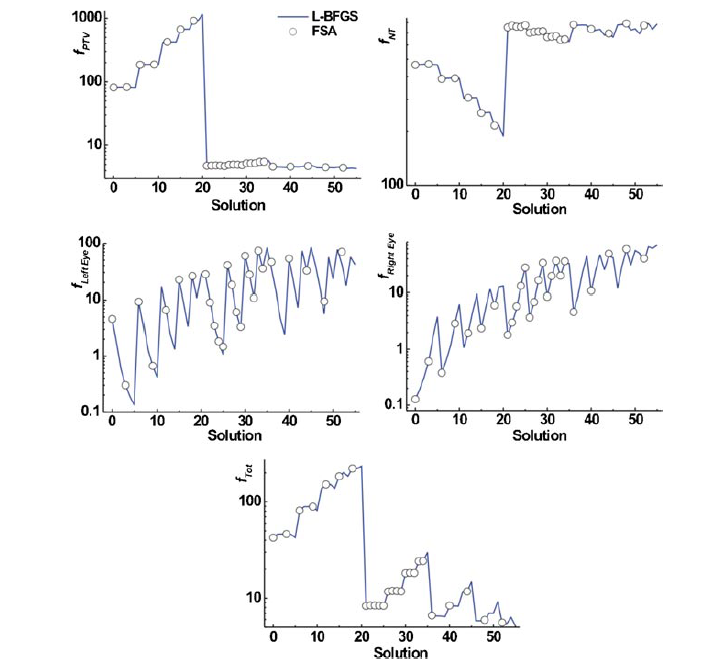
\includegraphics[width=0.8\textwidth]{graficos/Figura_12.PNG}
    \caption{Comparación de L-BFGS y FSA para el caso de tumor cerebral. Adaptado de Lahanas et al.\ (2003).}
    \label{fig:lbfgs_vs_fsa_cerebro}
\end{figure}

La figura~\ref{fig:lbfgs_vs_fsa_prostata} muestra la comparación para el caso de próstata, donde FSA requirió más de 10 horas por optimización. Vemos que se mantiene la coincidencia entre ambos métodos, incluso aunque sea un problema con más funciones objetivo.

\begin{figure}[H]
    \centering
    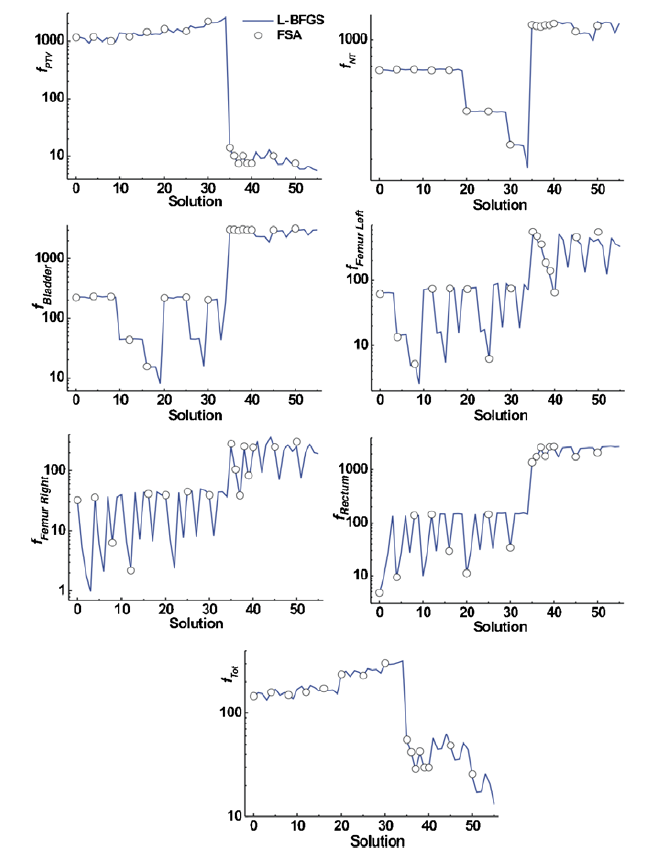
\includegraphics[width=0.85\textwidth]{graficos/Figura_13.PNG}
    \caption{Comparación de L-BFGS y FSA para el caso de cáncer de próstata. Adaptado de Lahanas et al.\ (2003).}
    \label{fig:lbfgs_vs_fsa_prostata}
\end{figure}

En conjunto, las tres comparaciones dejan probado que L-BFGS obtiene soluciones globalmente óptimas en todos los casos analizados, con una diferencia de aproximadamente tres órdenes de magnitud en tiempo de cómputo respecto de FSA.

\subsection{Optimización multiobjetivo: frente de Pareto}

Una vez establecido que el método es confiable, se generaron conjuntos de soluciones Pareto para cada caso, variando los vectores de pesos \(\lambda_m\).

\subsubsection*{Caso fantoma con PTV en forma de C}

La figura~\ref{fig:pareto_c} muestra las tres proyecciones bidimensionales del frente de Pareto tridimensional \((F_{\text{PTV}}, F_{\text{NT}}, F_{\text{OAR}})\). Cada punto representa una solución no dominada: ningún plan puede mejorar en uno de los objetivos sin empeorar en al menos otro. La proyección \((F_{\text{PTV}}, F_{\text{NT}})\) muestra que a medida que la varianza de dosis en el PTV se hace mínima (\(F_{\text{PTV}} \approx 5{,}7\)), la varianza en el tejido sano aumenta hacia \(F_{\text{NT}} \approx 2370\). Esto refleja que no existe ninguna configuración de beamlets que logre irradiar mucho al tumor sin irradiar órganos cercanos. El gráfico incluye dos conjuntos de soluciones: 1891 soluciones con \(s=1\) (pesos uniformes) y 136 soluciones con \(s=100\) (peso para el PTV amplificado). Las soluciones con \(s=1\) cubren una extensa región, pero incluyen zonas que son clínicamente inaceptables; las soluciones con \(s=100\) se concentran en la región de PTV  bajo, que es la opción clínicamente relevante.

\begin{figure}[H]
    \centering
    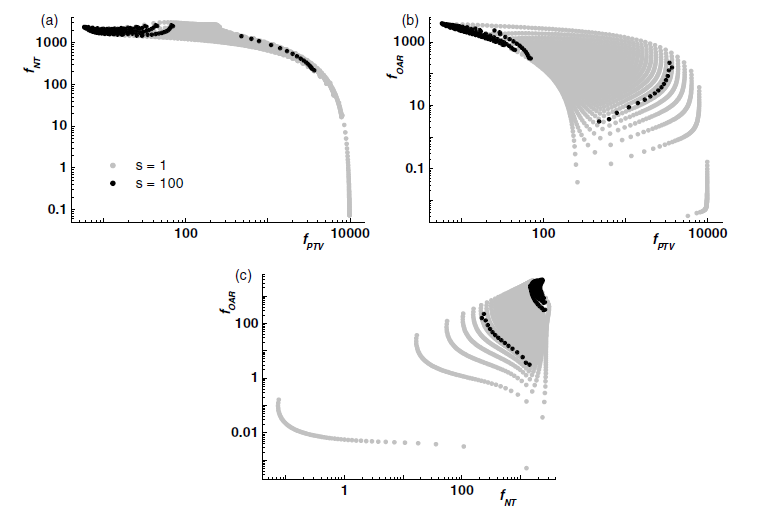
\includegraphics[width=0.85\textwidth]{graficos/Figura_16.PNG}
    \caption{Proyecciones bidimensionales del frente de Pareto tridimensional para el caso con PTV en forma de C: \((F_{\text{PTV}}, F_{\text{NT}})\), \((F_{\text{PTV}}, F_{\text{OAR}})\) y \((F_{\text{NT}}, F_{\text{OAR}})\). Se muestran 1891 soluciones con \(s=1\) y 136 soluciones con \(s=100\). Adaptado de Lahanas et al.\ (2003).}
    \label{fig:pareto_c}
\end{figure}

La figura~\ref{fig:dvh_c} muestra los DVH para el conjunto de soluciones generadas. Cada curva representa un plan de tratamiento diferente: el eje horizontal es la dosis normalizada respecto de la prescrita (\(D/D_{\text{ref}}\)) y el eje vertical es el porcentaje del volumen del órgano que recibe al menos esa dosis. Para el PTV, todas las soluciones filtradas presentan DVH similares, con la curva cayendo abruptamente cerca de \(D/D_{\text{ref}} = 1\), lo que indica cobertura casi completa a la dosis prescrita. Se observa además que usar \(D_{\text{crit}} = 0\) (columna derecha) permite que haya más soluciones para el OAR en comparación a cuando \(D_{\text{crit}} = 0{,}5\,D_{\text{ref}}\) (columna izquierda). Esto se debe a que, al no imponer un umbral de penalización, el algoritmo explora toda la región del espacio de dosis y puede encontrar planes con menor dosis en el OAR.

\begin{figure}[H]
    \centering
    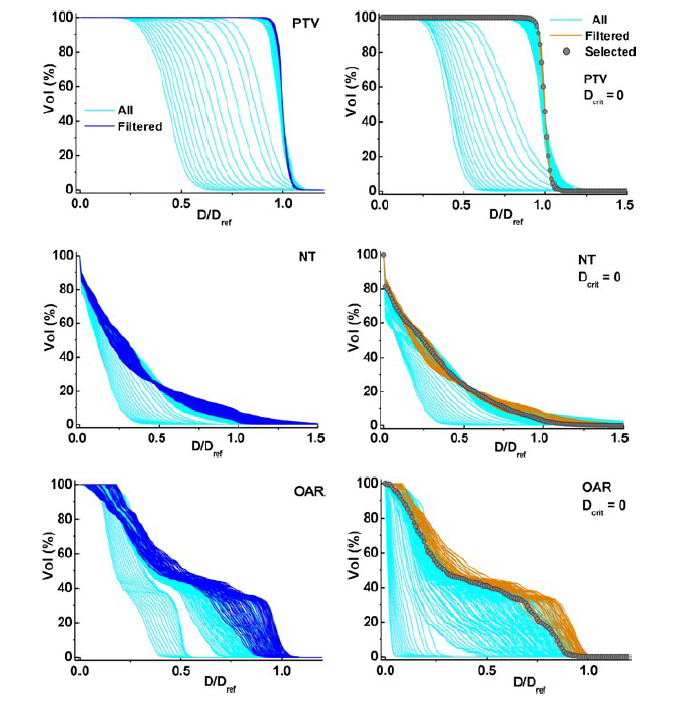
\includegraphics[width=0.85\textwidth]{graficos/Figura_18.PNG}
    \caption{DVHs de 136 soluciones para el PTV, el tejido sano y el OAR en el caso con PTV en forma de C, con \(D_{\text{crit}} = 0{,}5\,D_{\text{ref}}\) (izquierda) y \(D_{\text{crit}} = 0\) (derecha). Adaptado de Lahanas et al.\ (2003).}
    \label{fig:dvh_c}
\end{figure}

\subsubsection*{Caso tumor cerebral}

Para el caso de tumor cerebral, la figura~\ref{fig:dvh_cerebro} muestra los DVH para 165 soluciones. Se observa que, a diferencia del caso anterior, el espectro de soluciones es más amplio, por lo que la dosis puede reducirse en ambos ojos sin comprometer la dosis sobre el PTV, que permanece prácticamente constante entre soluciones. La comparación entre los casos con \(D_{\text{crit}} = 63{,}4\%\,D_{\text{ref}}\) (izquierda) y \(D_{\text{crit}} = 0\) (derecha) muestra nuevamente que cuando no hay umbral, se producen soluciones con menor dosis en los OARs.

\begin{figure}[H]
    \centering
    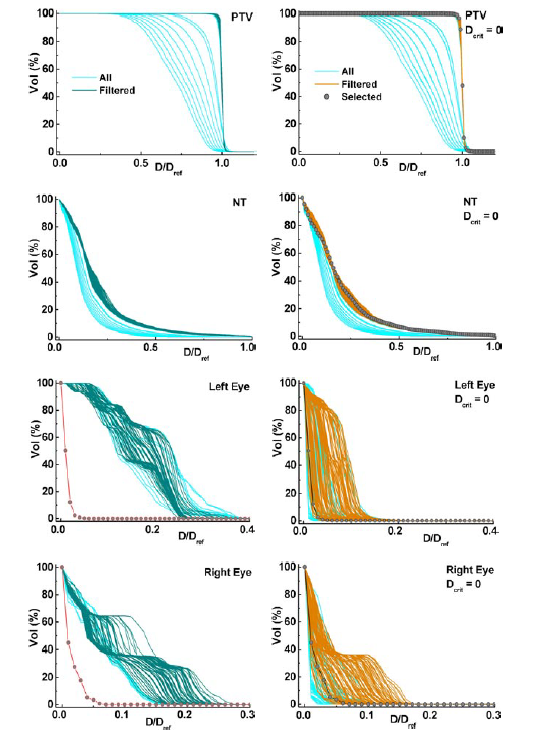
\includegraphics[width=0.85\textwidth]{graficos/Figura_19.PNG}
    \caption{DVHs de 165 soluciones para el PTV, el tejido sano y los OARs en el caso de tumor cerebral, con \(D_{\text{crit}} = 63{,}4\%\,D_{\text{ref}}\) (izquierda) y \(D_{\text{crit}} = 0\) (derecha) para ambos ojos. Adaptado de Lahanas et al.\ (2003).}
    \label{fig:dvh_cerebro}
\end{figure}

\subsubsection*{Caso cáncer de próstata}

La figura~\ref{fig:pareto_prostata} muestra las proyecciones del frente de Pareto sobre \((F_{\text{PTV}}, F_{\text{OAR}})\) para cada uno de los cuatro OARs. Se observa que para vejiga y recto, al reducir la varianza en el PTV aumenta mucho la dosis en estas estructuras. En cambio, las cabezas femorales presentan una correlación más débil, dado que están colocadas lateralmente respecto del volumen de tratamiento. La escala es doblemente logarítmica para revelar la estructura fina del frente en las zonas de bajo \(F_{\text{PTV}}\).

\begin{figure}[H]
    \centering
    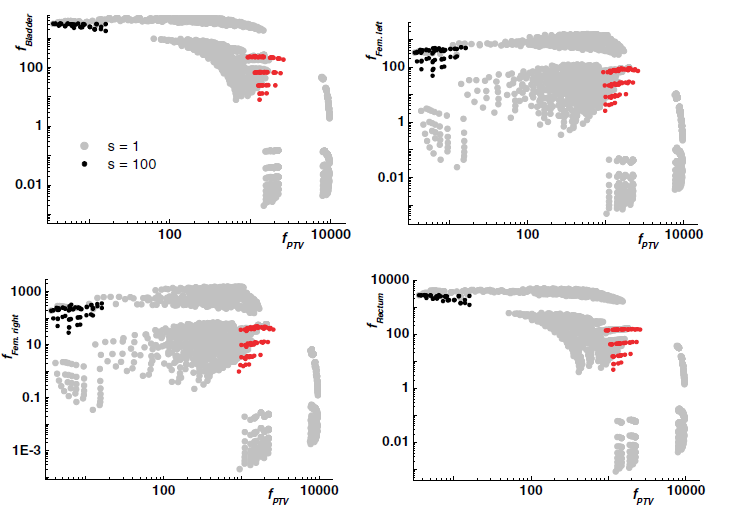
\includegraphics[width=0.85\textwidth]{graficos/Figura_21.PNG}
    \caption{Proyecciones del frente de Pareto para el cáncer de próstata. Hay 2002 soluciones con \(s=1\) y 126 soluciones con \(s=100\). Adaptado de Lahanas et al.\ (2003).}
    \label{fig:pareto_prostata}
\end{figure}

La figura~\ref{fig:dvh_prostata} muestra los DVH para 126 soluciones del caso de próstata. La cobertura máxima del PTV al 95\% de la dosis prescrita alcanzó el 98,8\% (resultado óptimo). Para vejiga y recto, el espectro de DVH es amplio, por lo que el planificador tiene un margen grande de elección para priorizar uno u otro órgano según el caso clínico en particular. Al igual que en los casos anteriores, el uso de \(D_{\text{crit}} = 0\) produce un espectro más amplio, que incluye soluciones de menor dosis en los OARs.

\begin{figure}[H]
    \centering
    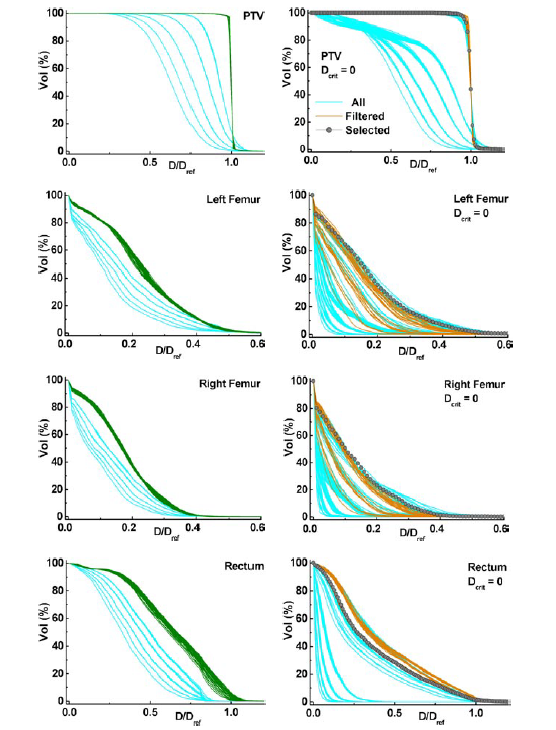
\includegraphics[width=0.85\textwidth]{graficos/Figura_22.PNG}
    \caption{DVHs de 126 soluciones para el PTV y los OARs en el caso de cáncer de próstata. Adaptado de Lahanas et al.\ (2003).}
    \label{fig:dvh_prostata}
\end{figure}